\documentclass[manuscript,anonymous]{acmart}
\usepackage[utf8]{inputenc}
\usepackage{algpseudocode} % for pseudocode
\usepackage{tikz} % for figures
\usepackage{subcaption} % for subfigures

\begin{document}
\title{Brief Announcement: Byzantine Eventual Consistency}
\author{Martin Kleppmann}
\email{mk428@cst.cam.ac.uk}
\orcid{0000-0001-7252-6958}
\affiliation{%
  \institution{University of Cambridge}
  \streetaddress{15 JJ Thomson Avenue}
  \city{Cambridge}
  \postcode{CB3 0FD}
  \country{UK}
}

\author{Heidi Howard}
\email{hh360@cst.cam.ac.uk}
\orcid{0000-0001-5256-7664}
\affiliation{%
  \institution{University of Cambridge}
  \streetaddress{15 JJ Thomson Avenue}
  \city{Cambridge}
  \postcode{CB3 0FD}
  \country{UK}
}

\begin{abstract}
    If $1/3$ or more processes may be faulty, a Byzantine agreement algorithm cannot make any consistency guarantees.
    However, in such situations we can still guarantee a weaker consistency model, which we call Byzantine Eventual Consistency (BEC).
    We define BEC and introduce an algorithm that ensures this consistency model, even in a system with arbitrarily many faulty processes.
\end{abstract}
\maketitle

\section{Introduction}

Byzantine agreement assumes that at most $f$ out of $n$ processes are Byzantine-faulty.
It is well established that without synchrony, Byzantine agreement is impossible if $n\leq3f$~\cite{Lamport:1982,Dwork:1988,Fischer:1985}.
If more than $f$ processes are faulty, neither safety nor liveness can be guaranteed.
This is a problem because the $f$-faulty assumption is not always a realistic threat model.
Byzantine failures are not necessarily independent: if an adversary can compromise one of the processes (e.g. due to a software vulnerability), it is likely that they can compromise a majority of processes, since they are likely to all be running the same software. 
Similarly, non-malicious software bugs are likely to affect many of the processes at once.
Moreover, in some systems, the adversary may be able to spawn a large number of processes, and thus create a majority of Byzantine-faulty processes (this is known as a Sybil attack~\cite{Douceur:2002jr}).

This state of affairs raises the question: if Byzantine agreement cannot be achieved in the face of arbitrary numbers of Byzantine-faulty processes, what consistency model \emph{can} we achieve under that assumption?

In this paper we propose \emph{Byzantine Eventual Consistency} (BEC), a consistency model that can be achieved regardless of the number of Byzantine-faulty processes.
We define BEC in Section~\ref{sec:properties}, and in Section~\ref{sec:algorithm} we describe an algorithm that achieves BEC.
The idea behind BEC is that each process acts as a replica of some shared state, and that any two correct replicas converge towards the same state as they communicate.
This property holds even if replicas also communicate with arbitrarily many Byzantine-faulty processes in the system.
Essentially, we need to ensure that faulty replicas cannot corrupt the state of correct replicas.

\section{Defining Byzantine Eventual Consistency}\label{sec:properties}

Byzantine agreement is often used to decide an append-only log of values for state machine replication~\cite{Schneider:1990} (SMR) and thus requires that the following properties hold:

\begin{description}
\item[Validity:] Any value decided by a correct process must have been proposed by one of the processes.
\item[Agreement:] When any two correct processes decide a value for a certain position in the log, those decided values are the same.
\item[Liveness:] For any value proposed, correct processes will eventually decide that value for some position in the log.
\end{description}

Agreement and liveness assume that no more than $f$ processes are Byzantine-faulty and liveness also assumes partial synchrony~\cite{Dwork:1988}.

We can define a similar set of properties for Byzantine Eventual Consistency (BEC).
These properties are weaker, but they can be satisfied without making any assumptions about the number of faulty processes or the synchrony model.
For generality, we assume each process locally maintain a monotonically growing set of updates $\mathcal{U}$.
We later discuss how this set of updates can be utilised to implement SMR.

\begin{description}
\item[Validity:] Any update in the set of updates of a correct process must have been proposed by one of the processes.
\item[Convergence:] When any two correct processes finish communicating, their sets of updates are the same.
\item[Liveness:] Assuming that any two correct processes will eventually finish communicating, a update proposed by one process will eventually be in the set of updates for all correct processes.
\end{description}

\section{Reconciliation algorithms}\label{sec:algorithm}

When two processes $p$ and $q$ communicate, and each process initially has updates $\mathcal{U}_p$ and $\mathcal{U}_q$ respectively, a reconciliation algorithm should ensure that both processes converge to the same set $\mathcal{U}_q \cup \mathcal{U}_q$.
The simplest reconciliation algorithm is for $p$ to send the entire set $\mathcal{U}_p$ to $q$, and for $q$ to send $\mathcal{U}_q$ to $p$, so that both processes can compute $\mathcal{U}_q \cup \mathcal{U}_q$.
However, if the sets have many elements in common, this algorithm transmits a large amount of data unnecessarily.

In more efficient reconciliation algorithms, processes often rely on vector clocks to determine which updates to send to each other (TODO reference?).
However, vector clocks are not suitable in a Byzantine setting, because a faulty node could send contradictory updates to different processes under the same vector timestamp, causing two processes to have the same vector timestamps, but inconsistent sets of updates.
Therefore we introduce a reconciliation algorithm that cannot be corrupted by faulty processes.

Let the set of updates $\mathcal{U}$ be a set of pairs $(v, \mathit{hs})$, where $v$ is any value, and $\mathit{hs}$ is a set of hashes produced by a cryptographic hash function $H(\cdot)$, such as SHA-256.
We assume that $H$ is collision-resistant (i.e.\ it is computationally infeasible to find distinct $x$ and $y$ such that $H(x) = H(y)$).

Say $\mathcal{U}$ contains updates $A = (v_A, \mathit{hs}_A)$ and $B = (v_B, \mathit{hs}_B)$, where $H(A) \in \mathit{hs}_B$.
Then we call $A$ a \emph{predecessor} of $B$, and $B$ a \emph{successor} of $A$.
Define a graph with a vertex for each update in $\mathcal{U}$, and a directed edge from each update to each of its predecessors.
We can assume that this graph is acyclic because the presence of a cycle would imply knowledge of a collision in the hash function.
Fig.~\ref{fig:example-dags} shows examples of such graphs.

Let $\mathrm{succ}^1(u)$ be the set of successors of update $u$, let $\mathrm{succ}^2(u)$ be the successors of the successors of $u$, and so on, and define $\mathrm{succ}^*(u)$ to be the transitive closure:
\[
\mathrm{succ}^i(u) =
\begin{cases}
\{( v, \mathit{hs}) \in \mathcal{U} \mid H(u) \in \mathit{hs}\} & \text{ for } i=1 \\
\bigcup_{u' \in \mathrm{succ}^1(u)} \mathrm{succ}^{i-1}(u') & \text{ for } i>1
\end{cases}
\hspace{60pt}
\mathrm{succ}^*(u) = \bigcup_{i \ge 1} \mathrm{succ}^i(u)
\]

When one process connects to another, both processes execute the algorithm in Fig.~\ref{fig:algorithm}.
We will illustrate the operation of this algorithm using the example in Fig.~\ref{fig:example-dags}; the messages sent in the course of the execution are shown in Fig.~\ref{fig:messages}.

\begin{figure}[p]
\captionsetup{justification=raggedright,singlelinecheck=false}
\begin{minipage}{0.5\linewidth}
    \hrule\vspace{4pt}
    \algblockdefx{On}{EndOn}[1]{\textbf{on} #1 \textbf{do}}{\textbf{end on}}
    \begin{algorithmic}[1]
    \On{connecting to another process}
        \State $\mathit{received} := \{\}$ \Comment{connection-local variable}
        \State $\mathit{heads} := \{u \in \mathcal{U} \mid \nexists (v, \mathit{hs}) \in \mathcal{U}.\; H(u) \in \mathit{hs}\}$
        \State \textbf{send} $\langle\mathsf{updates}: \mathit{heads}\rangle$
    \EndOn\vspace{10pt}
    \On{receiving $\langle\mathsf{updates}: \mathit{new}\rangle$}
        \State $\mathit{received} := \mathit{received} \,\cup\, \mathit{new}$
        \State $\mathit{reply} := \bigcup_{u \in \mathit{new}} \mathrm{succ}^*(u)$
        \If{$\mathit{reply} \neq \{\}$}
            \State \textbf{send} $\langle\mathsf{updates}: \mathit{reply}\rangle$
        \EndIf
        \State $\mathit{missing} := \{h \mid \exists (v, \mathit{hs}) \in \mathit{received}.\; h \in \mathit{hs} \;\wedge$
        \State \hspace{55pt}$\; \nexists u \in (\mathcal{U} \cup \mathit{received}).\; H(u) = h\}$
        \If{$\mathit{missing} = \{\}$}
            \State $\mathcal{U} := \mathcal{U} \cup \mathit{received}$
            \State \textbf{finish protocol}
        \Else
            \State \textbf{send} $\langle\mathsf{needs}: \mathit{missing}\rangle$
        \EndIf
    \EndOn\vspace{10pt}
    \On{receiving $\langle\mathsf{needs}: \mathit{missing}\rangle$}
        \State \textbf{send} $\langle\mathsf{updates}: \{u \in \mathcal{U} \mid H(u) \in \mathit{missing}\}\rangle$
    \EndOn
    \end{algorithmic}
    \vspace{4pt}\hrule
    \caption{A reconciliation algorithm that exchanges updates between two processes.}\label{fig:algorithm}
\end{minipage}\hfill
\begin{minipage}{0.4\linewidth}
    \begin{subfigure}{\textwidth}
    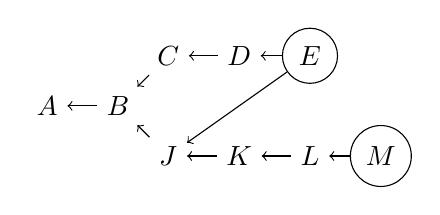
\begin{tikzpicture}[node distance=0.9cm]

% nodes
\node (a) {$A$};
\node (b) [right of=a] {$B$};
\node (c) [above right of=b] {$C$};
\node (d) [right of=c] {$D$};
\node (e) [right of=d,draw,circle] {$E$};
\node (j) [below right of=b] {$J$};
\node (k) [right of=j] {$K$};
\node (l) [right of=k] {$L$};
\node (m) [right of=l,draw,circle] {$M$};

% arrows
\draw[<-] (a) -- (b);
\draw[<-] (b) -- (c);
\draw[<-] (c) -- (d);
\draw[<-] (d) -- (e);
\draw[<-] (j) -- (e);
\draw[<-] (b) -- (j);
\draw[<-] (j) -- (k);
\draw[<-] (k) -- (l);
\draw[<-] (l) -- (m);
\end{tikzpicture}
    \caption{Graph of updates at $p$ before reconciliation}
    \end{subfigure}\\[35pt]
    \begin{subfigure}{\textwidth}
    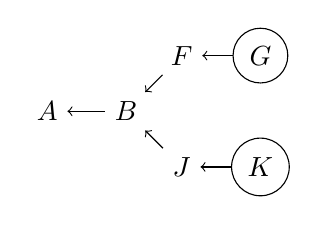
\begin{tikzpicture}

% nodes
\node (a) {$A$};
\node (b) [right of=a] {$B$};
\node (f) [above right of=b] {$F$};
\node (g) [right of=f,circle,draw] {$G$};
\node (j) [below right of=b] {$J$};
\node (k) [right of=j,circle,draw] {$K$};

% arrows
\draw[<-] (a) -- (b);
\draw[<-] (b) -- (f);
\draw[<-] (f) -- (g);
\draw[<-] (b) -- (j);
\draw[<-] (j) -- (k);
\end{tikzpicture}
    \caption{Graph of updates at $q$ before reconciliation}
    \end{subfigure}\\[35pt]
    \begin{subfigure}{\textwidth}
    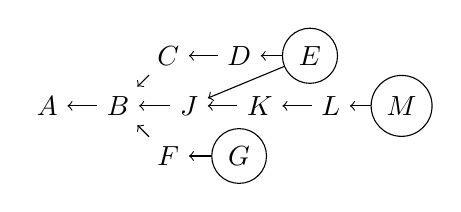
\begin{tikzpicture}[node distance=0.9cm]

% nodes
\node (a) {$A$};
\node (b) [right of=a] {$B$};
\node (c) [above right of=b] {$C$};
\node (d) [right of=c] {$D$};
\node (e) [right of=d,draw,circle] {$E$};
\node (j) [right of=b] {$J$};
\node (k) [right of=j] {$K$};
\node (l) [right of=k] {$L$};
\node (m) [right of=l,draw,circle] {$M$};
\node (f) [below right of=b] {$F$};
\node (g) [right of=f,draw,circle] {$G$};

% arrows
\draw[<-] (a) -- (b);
\draw[<-] (b) -- (c);
\draw[<-] (c) -- (d);
\draw[<-] (d) -- (e);
\draw[<-] (b) -- (j);
\draw[<-] (j) -- (e);
\draw[<-] (j) -- (k);
\draw[<-] (k) -- (l);
\draw[<-] (l) -- (m);
\draw[<-] (b) -- (f);
\draw[<-] (f) -- (g);
\end{tikzpicture}
    \caption{Graph of updates at $p$ and $q$ after reconciliation}
    \end{subfigure}
    \caption{Example DAGs of updates. Arrows represent an update referencing the hash of its predecessor, and heads (updates with no successors) are marked with circles.}
    \label{fig:example-dags}
\end{minipage}
\end{figure}

\begin{figure}[p]
    \centering
    \vspace{0.5cm}
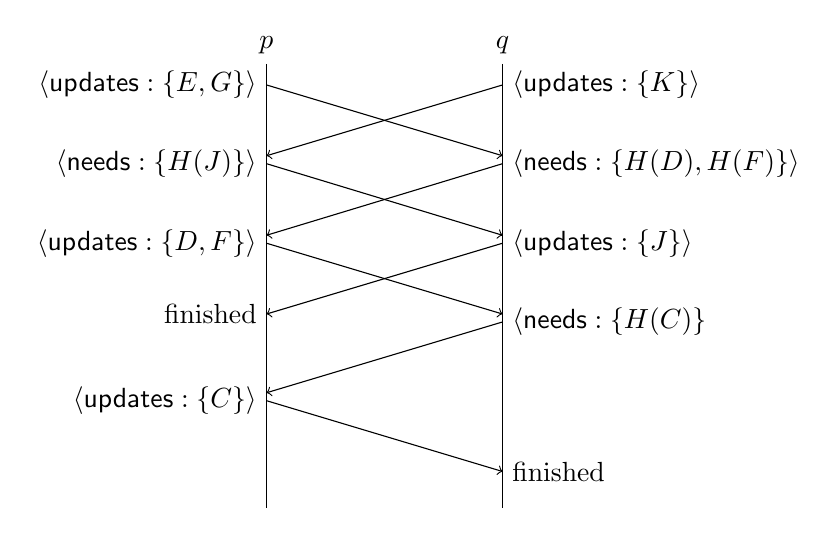
\begin{tikzpicture}
\def\width{3cm}
\def\latency{1cm}
\def\spacing{0.1cm}
\def\length{6cm}
\def\startdelay{0.5cm}

% Timelimes
\node (p1-start) at (0,0) {$p$};
\node (p2-start) at (\width,0) {$q$};
\node (p1-end) at (0,-\length) {};
\node (p2-end) at (\width,-\length) {};
\draw (p1-start) -- (p1-end);
\draw (p2-start) -- (p2-end);

% Messages
\draw[->] (0,-\startdelay) node[left] {$\langle\mathsf{updates}: \{E,G\}\rangle$} -- (\width,\spacing-\startdelay-\latency);
\draw[->] (\width,-\startdelay) node[right] {$\langle\mathsf{updates}: \{K\}\rangle$} -- (0,\spacing-\startdelay-\latency);

\draw[->] (\width, -\startdelay-\latency) node[right] {$\langle\mathsf{needs}: \{H(D), H(F)\}\rangle$} -- (0,\spacing-\startdelay-2.0\latency);
\draw[->] (0, -\startdelay-\latency) node[left] {$\langle\mathsf{needs}: \{H(J)\}\rangle$} -- (\width,\spacing-\startdelay-2.0\latency);

\draw[->] (0, -\startdelay-2.0\latency) node[left] {$\langle\mathsf{updates}: \{D, F\}\rangle$} -- (\width,\spacing-\startdelay-3.0\latency);
\draw[->] (\width, -\startdelay-2.0\latency) node[right] {$\langle\mathsf{updates}: \{J\}\rangle$} -- (0,\spacing-\startdelay-3.0\latency) node[left] {finished};

\draw[->] (\width, -\startdelay-3.0\latency) node[right] {$\langle\mathsf{needs}: \{H(C)\}$} -- (0,\spacing-\startdelay-4.0\latency);

\draw[->] (0, -\startdelay-4.0\latency) node[left] {$\langle\mathsf{updates}: \{C\}\rangle$} -- (\width,\spacing-\startdelay-5.0\latency) node[right] {finished};

\end{tikzpicture}
    \caption{Messages sent in the course of running the reconciliation algorithm in Fig.~\ref{fig:algorithm} with the example in Fig.~\ref{fig:example-dags}.}
    \label{fig:messages}
\end{figure}

Initially, when a connection is established between two processes, they send each other their \emph{heads}: that is, the updates in their local set $\mathcal{U}$ that have no successors (Fig.~\ref{fig:algorithm}, lines 3--4).
In the example of Fig.~\ref{fig:example-dags}, $p$ sends $E$ and $G$ to $q$, while $q$ sends $K$ to $p$.
Each process also initialises a variable $\mathit{received}$ to contain the set of updates received from the other process within the scope of this particular connection (lines 2 and 7).

On receiving the set of heads from the other process (line 6), the recipient first checks if its local set $\mathcal{U}$ contains successors for any of the sender's heads; if so, those successors, and any transitive successors, are sent immediately to the other process (lines 8--11).
By definition of $\mathit{heads}$, these successors are not yet known to the other process.

Next, we examine the hashes contained in the set of updates received from the other process, and identify any hashes for which we do not have a matching update (lines 12--13).
If there are no such hashes, we merge the set of received updates into $\mathcal{U}$ and conclude the protocol run (lines 14--16).
If there are unresolved hashes, we send a $\mathsf{needs}$ message to the other process, requesting the updates identified by those hashes (line 18).
The processes respond to such a $\mathsf{needs}$ message by returning all the matching updates in an $\mathsf{updates}$ message (lines 21--23).

In the example of Figs.~\ref{fig:example-dags} and~\ref{fig:messages}, when $q$ receives $\{E, G\}$, those updates contain hashes $H(D)$ and $H(F)$; since $q$ does not yet know either $D$ or $F$, it sends a $\mathsf{needs}$ message containing those hashes back to $p$.
In the opposite direction, when $p$ receives $\{K\}$ containing $H(J)$, $p$ needs to request $J$ from $q$.
In successive rounds of this protocol, the processes work their way from the heads backwards along the paths of predecessors, until they find the updates that are common ancestors of both processes' heads.
We show in the appendix that this algorithm ensures Byzantine Eventual Consistency.

\subsection{Optimisations}\label{sec:optimisations}

The algorithm in Fig.~\ref{fig:algorithm} is efficient in the sense that it does not send any updates that the other process already has, with the exception of updates sent in the initial $\mathit{heads}$ message.
Assuming that the number of heads is small compared to the total number of updates in $\mathcal{U}$, this is a performance improvement over sending the whole of $\mathcal{U}$.

In order to keep the number of heads small, whenever a correct process generates a new update $(v, \mathit{hs})$, it should set $\mathit{hs}$ to be the set of hashes of the current \emph{heads}:
$\mathit{hs} = \{H(u) \mid u \in \mathcal{U} \wedge \mathrm{succ}^1(u) = \{\}\,\}$.
% Alternative notation:
%$\mathit{hs} = \{H(u) \mid u \in \mathcal{U} \wedge \nexists (t, v, \mathit{hs}) \in \mathcal{U}.\; H(u) \in \mathit{hs}\}$
In this construction, the number of heads is bounded by the number of processes generating updates concurrently.
When a Byzantine-faulty process generates new updates, we cannot guarantee that it will follow this approach, and thus a faulty process may generate a large number of heads.
While this will affect the performance of the algorithm, it will not affect its correctness.

A downside of the algorithm in Fig.~\ref{fig:algorithm} is that the number of round trips required can be up to the length of the longest path in the graph.
In order to optimise this, we could change line 22 so that it sends not only the immediate updates identified by the hashes in the $\mathsf{needs}$ message, but also all of the predecessors of those updates, several levels deep.
The number of round-trips is then reduced proportionally to the number of predecessor levels, but the downside is that some of the predecessors may already be known to the recipient, and are thus transmitted unnecessarily.

To determine the number of predecessor levels to send in each round, as a rule of thumb, the size of the $\mathsf{updates}$ message should be approximately equal to the bandwidth-delay product of the connection between the two processes.
Thus, on a connection with low bandwidth and fast round-trips we will prefer to send many small messages, while on a connection with high bandwidth and slow round-trips we will batch the updates into a small number of large messages.

% Prevent unbounded storage growth
% Find last common ancestor by some kind of binary search; problem: graph of updates is not linear, so definition of half-way point is fiddly.

\section{State machine replication}

BEC can ensure convergence for any data structure that is a deterministic function of the set of updates $\mathcal{U}$.
We now show that State Machine Replication (SMR) is one such example.

We can implement such a BEC-SMR as follows: let each value consists of a pairs, $(t, op)$, where $t$ is a timestamp and $op$ is a operation for the state machine.
Any process may propose an operation $op$ to add to the log by generating $t$ and adding $(t, op)$ to $\mathcal{U}$.
The log is then simply the sequence of values obtained by sorting the elements in $\mathcal{U}$ by their timestamp, breaking ties by ordering on values.

% TODO should we say something about how a BEC log can be used? Something like state machine replication is still possible, but you have to have some kind of rollback/rewinding to deal with elements arriving out-of-order.


\section{Related Work}

Byzantine agreement~\cite{Lamport:1982} has been subject of extensive research and has seen a recent renewal of interest due to its application in blockchains~\cite{Bano:2019}.
Most Byzantine agreement algorithms assume that $n=3f+1$~\cite{Castro:1999,Cowling:2006,Kotla:2007,Aublin:2015,Yin:2019}, while others require that $n=5f+1$~\cite{Abd:2005,Martin:2006}.
Some take a different approach to bounding the number of failures: for example, Upright~\cite{Clement:2009} separates the number of crash failures ($u$) and Byzantine failures ($r$) and assumes $n=2u+r+1$.

% add paragraph on the other issues with byzantine agreement e.g. high latency (one or more round trips to most processes), poor availability (a process cannot add an update less it can communicate with most other processes), need for cypto keys (the issue of how to securely set these up is seldom discussed) 

Byzantine eventual consistency is based on \emph{Strong Eventual Consistency} (SEC)~\cite{Shapiro:2011un}, a non-Byzantine consistency model in which replicas eventually converge towards the same state.
Conflict-free Replicated Data Types (CRDTs) provide SEC by ensuring that whenever any two replicas have seen the same set of updates (possibly in a different order), those replicas are in the same state~\cite{Shapiro:2011un}.
We can strengthen CRDTs to provide Byzantine Eventual Consistency by making each operation an update, and using the algorithm of Section~\ref{sec:algorithm} to reconcile the sets of operations.

The hash chaining approach of our algorithm in Section~\ref{sec:algorithm} has similarities to a Git commit history (where each commit references the hashes of its predecessor commits), a blockchain~\cite{Bano:2019}, or a Merkle tree~\cite{Merkle:1987}.

% Roy Friedman and Roni Licher. Hardening Cassandra Against Byzantine Failures.
% https://arxiv.org/pdf/1610.02885.pdf

% Ali Shoker et al. As Secure as Possible Eventual Consistency: Work in Progress (PaPoC 2017)
% https://dl.acm.org/doi/10.1145/3064889.3064895

% Wenbing Zhao and Mamdouh Babi. Byzantine fault tolerant collaborative editing.
% https://pdfs.semanticscholar.org/587b/c024d5e877608c79f484112666489d90f041.pdf

% Git fetch negotiation algorithm, How does this compare to git fetch negotiation algorithms, default and skipping?  
% https://stackoverflow.com/questions/40484929/will-a-git-pull-develop-fetch-all-the-commits-reacheable-from-develop
% https://git-scm.com/docs/git-config#Documentation/git-config.txt-fetchnegotiationAlgorithm

% Comparison to Julien Quintard work on byzantine file systems https://www.repository.cam.ac.uk/bitstream/handle/1810/243442/thesis.pdf?sequence=1&isAllowed=y
% https://infinit.sh

% Comparison to irmin
% https://mirage.github.io/irmin/irmin/Irmin/index.html#syncing-with-a-remote
% https://github.com/mirage/irmin/blob/master/src/irmin/sync_ext.ml#L86-L123

% Comparision to byzantine quorums
% http://www.cs.cornell.edu/courses/cs5414/2017fa/papers/bquorum-dc.pdf

% Comparision to byz chain replication
% https://link.springer.com/chapter/10.1007/978-3-642-35476-2_24

\section{Summary}

\begin{acks}
Martin Kleppmann is supported by a Leverhulme Trust Early Career Fellowship, and by the Isaac Newton Trust.
\end{acks}

\bibliographystyle{ACM-Reference-Format}
\bibliography{references}

\appendix
\section{Correctness of the reconciliation algorithm}
\begin{theorem}
The algorithm in Fig.~\ref{fig:algorithm} ensures Byzantine Eventual Consistency.
\end{theorem}
\begin{proof}[Proof sketch.]
TODO

% If the communication is between a correct and a Byzantine-faulty replica, the faulty replica can obviously add updates to the set or omit updates from those sent to the correct replica.
% But the faulty replica cannot corrupt the correct replica's state in a way that would prevent the correct replica from later synchronising its set of updates with another correct replica.

\end{proof}
\end{document}
